\documentclass{article}
\usepackage[utf8]{inputenc}
\usepackage{fancyhdr}
\usepackage{graphicx}
\usepackage{pdflscape}
\usepackage[margin=0.75in]{geometry}
 
\pagestyle{fancy}
\fancyhf{}
\rhead{Rachel LeCover}
\lhead{Biokinetics Problem Set 1}
\rfoot{Page \thepage}
 
\begin{document}
 
\section*{Problem 1}
I adjusted the control term following the logic presented by Moon et al in the supplemental material to "Genetic programs constructed from layered logic gates in single cells". I decided that there were three possible states-gene, open gene, and open gene with polymerase. I assumed that transcription could only occur when the open gene and polymerase were present. Therefore, I wrote a control term as
\begin{equation}
u_j = \frac{k_2f_{TL}}{1+k_2f_{TL}+k_3f_T}
\end{equation}

where $f_{TL}$ gives the fraction of the time where the polymerase is bound to the open gene, and $f_T$ is $1-f_{TL}$. The $k$s represent weights. Using this control term, and the formulation given in lecture for transcription, I produced a graph showing transcription rates for the two cases, Figure \ref{fig:P1Transcription}

\begin{figure}[!htb]
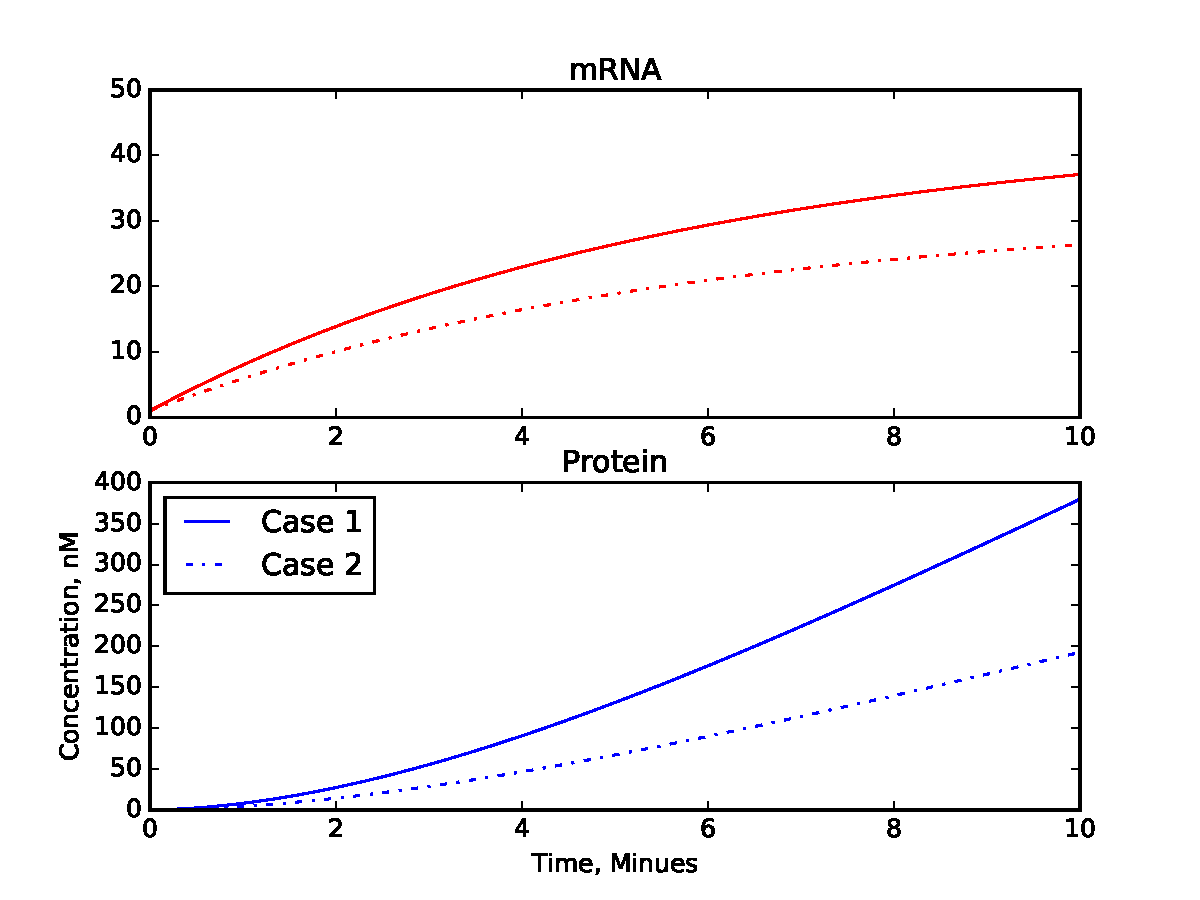
\includegraphics[width=12cm]{../Problem1/Problem1NotQuiteLinear}
\caption{Amounts of mRNA and protein produced with modified control term. To differentiate the two cases, when the gene and RNAP are incubated together (case 1), I made $k_2$ large, to heavily weight the state of bound open gene complex to promoter and in the case where no gene was present (case 2), I made $k_3$ large to account for a large population of the unbound state.}
\label{fig:P1Transcription}
\end{figure}
In my formulation, since gene length is not accounted for in the control term, it appears in the denominator of the expression for the transcription rate. 
\begin{equation}
r_{Tj} = \bar{r_{Tj}}u_j, 
\bar{r_{Tj}}= k_TR_T\frac{L_T}{L_{Tj}}\frac{G_j}{K_{Tj} + G_j}
\end{equation}
\begin{figure}[!htb]
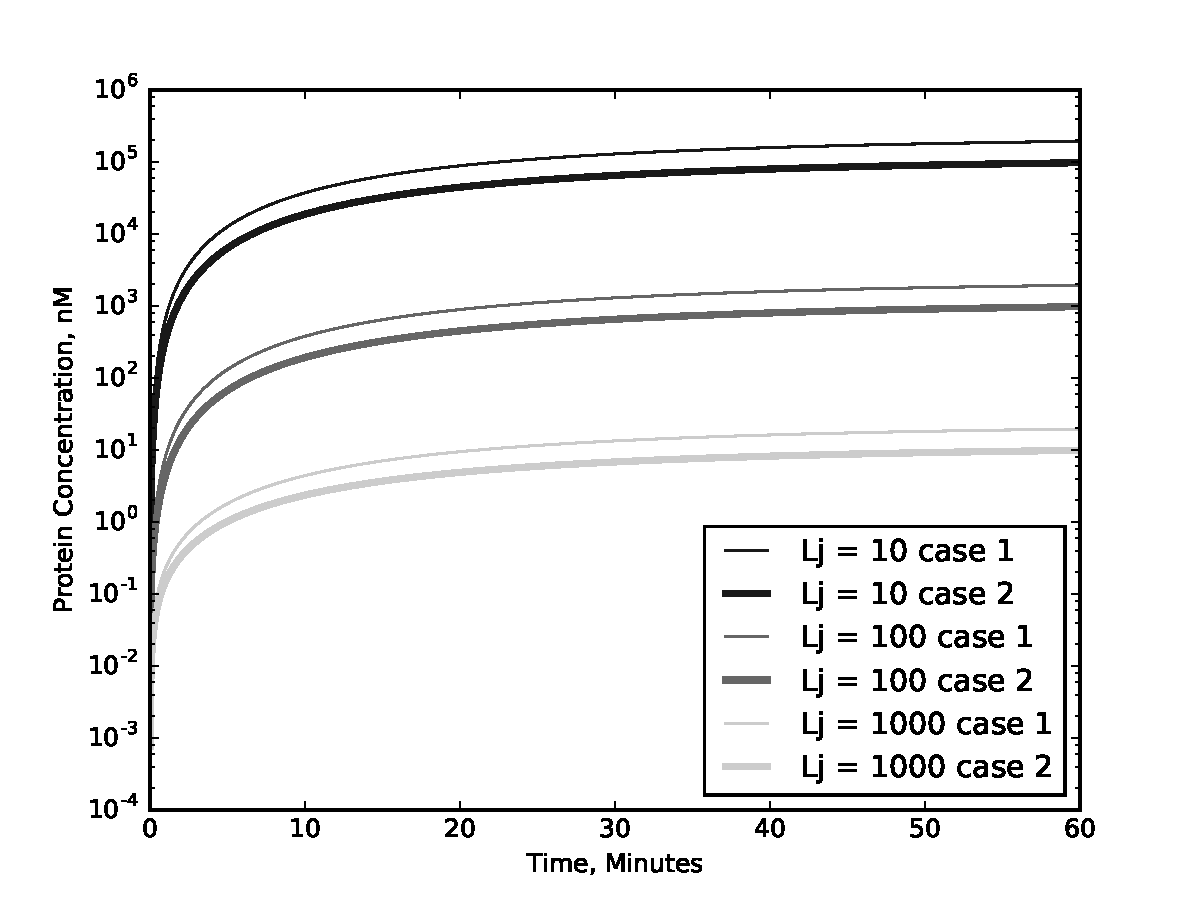
\includegraphics[width=12cm]{../Problem1/EffectsOfGeneLength}
\caption{Increasing the gene length dramatically decreases the amount of protein produced, as a log scale is necessary to capture the differences in protein levels on one plot}
\label{fig:P1GeneLen}
\end{figure}

So, as gene length increases, the rate of transcription decreases, as does the rate of translation due to the longer mRNA produced by longer genes, resulting in lower protein levels, as shown in Figure \ref{fig:P1GeneLen}. 
\newpage 
\section*{Problem 2}
At steady state, the protein levels are largely controlled by the weights in the control terms, as shown in Figure \ref{fig:P2SS}, as well as the global rate constants for transcription and translation. Specifically, other than the global parameters, the level of P1 largely depends on the weight with which RNA polymerase binds to its mRNA. The level of P2 depends on the strength of the interaction between P1 and P2. The amount of P3 depends on its interaction with P2. During induction the rate constants for transcription and translation as well as the rnapII concentration and ribosome concentration play a large role in the system response, as shown in Figure \ref{fig:P2Induced}. When a gene is being induced, the weights of the genes on each other become less important. The species-species and parameter-parameter interactions are shown in the supplemental material.

\begin{figure}[h]
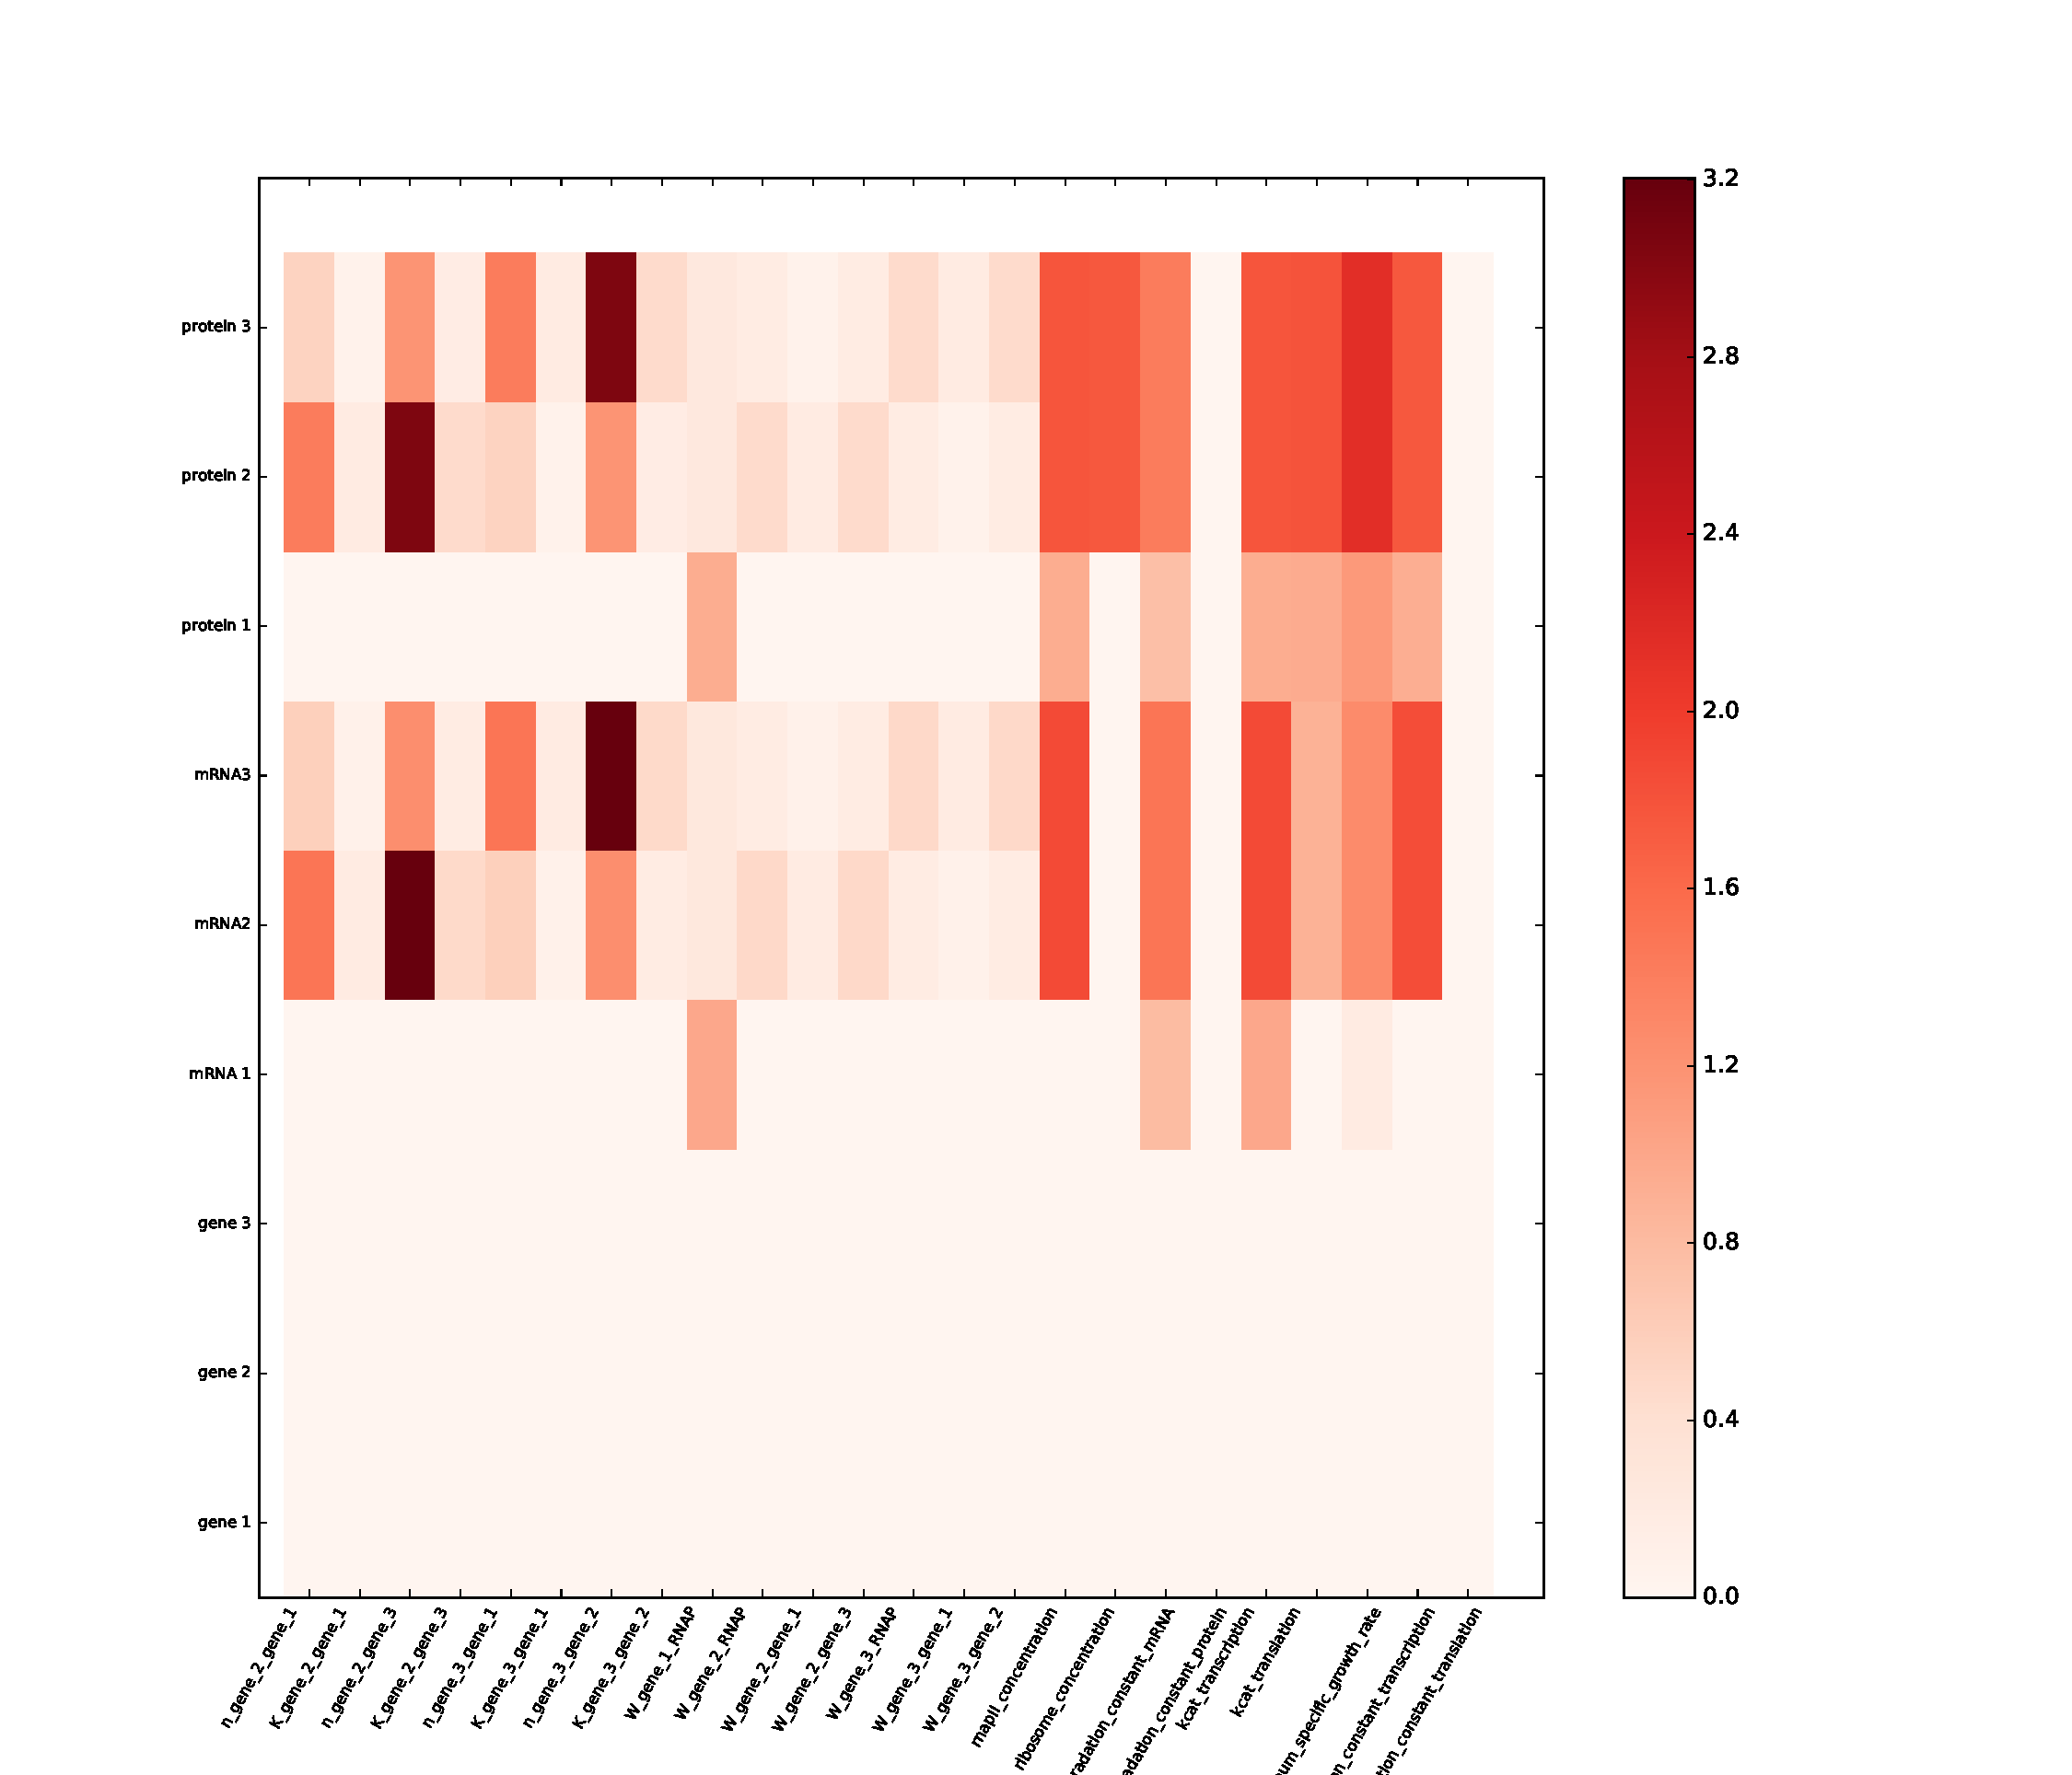
\includegraphics[width=12cm]{../ThreeGeneRachelV2/figures/ParameterSpeciesInteractionsFrom0to10}
\caption{Heat map produced time averaged sensitivity array of three gene network at steady state}
\label{fig:P2SS}
\end{figure}

\begin{figure}[!htb]
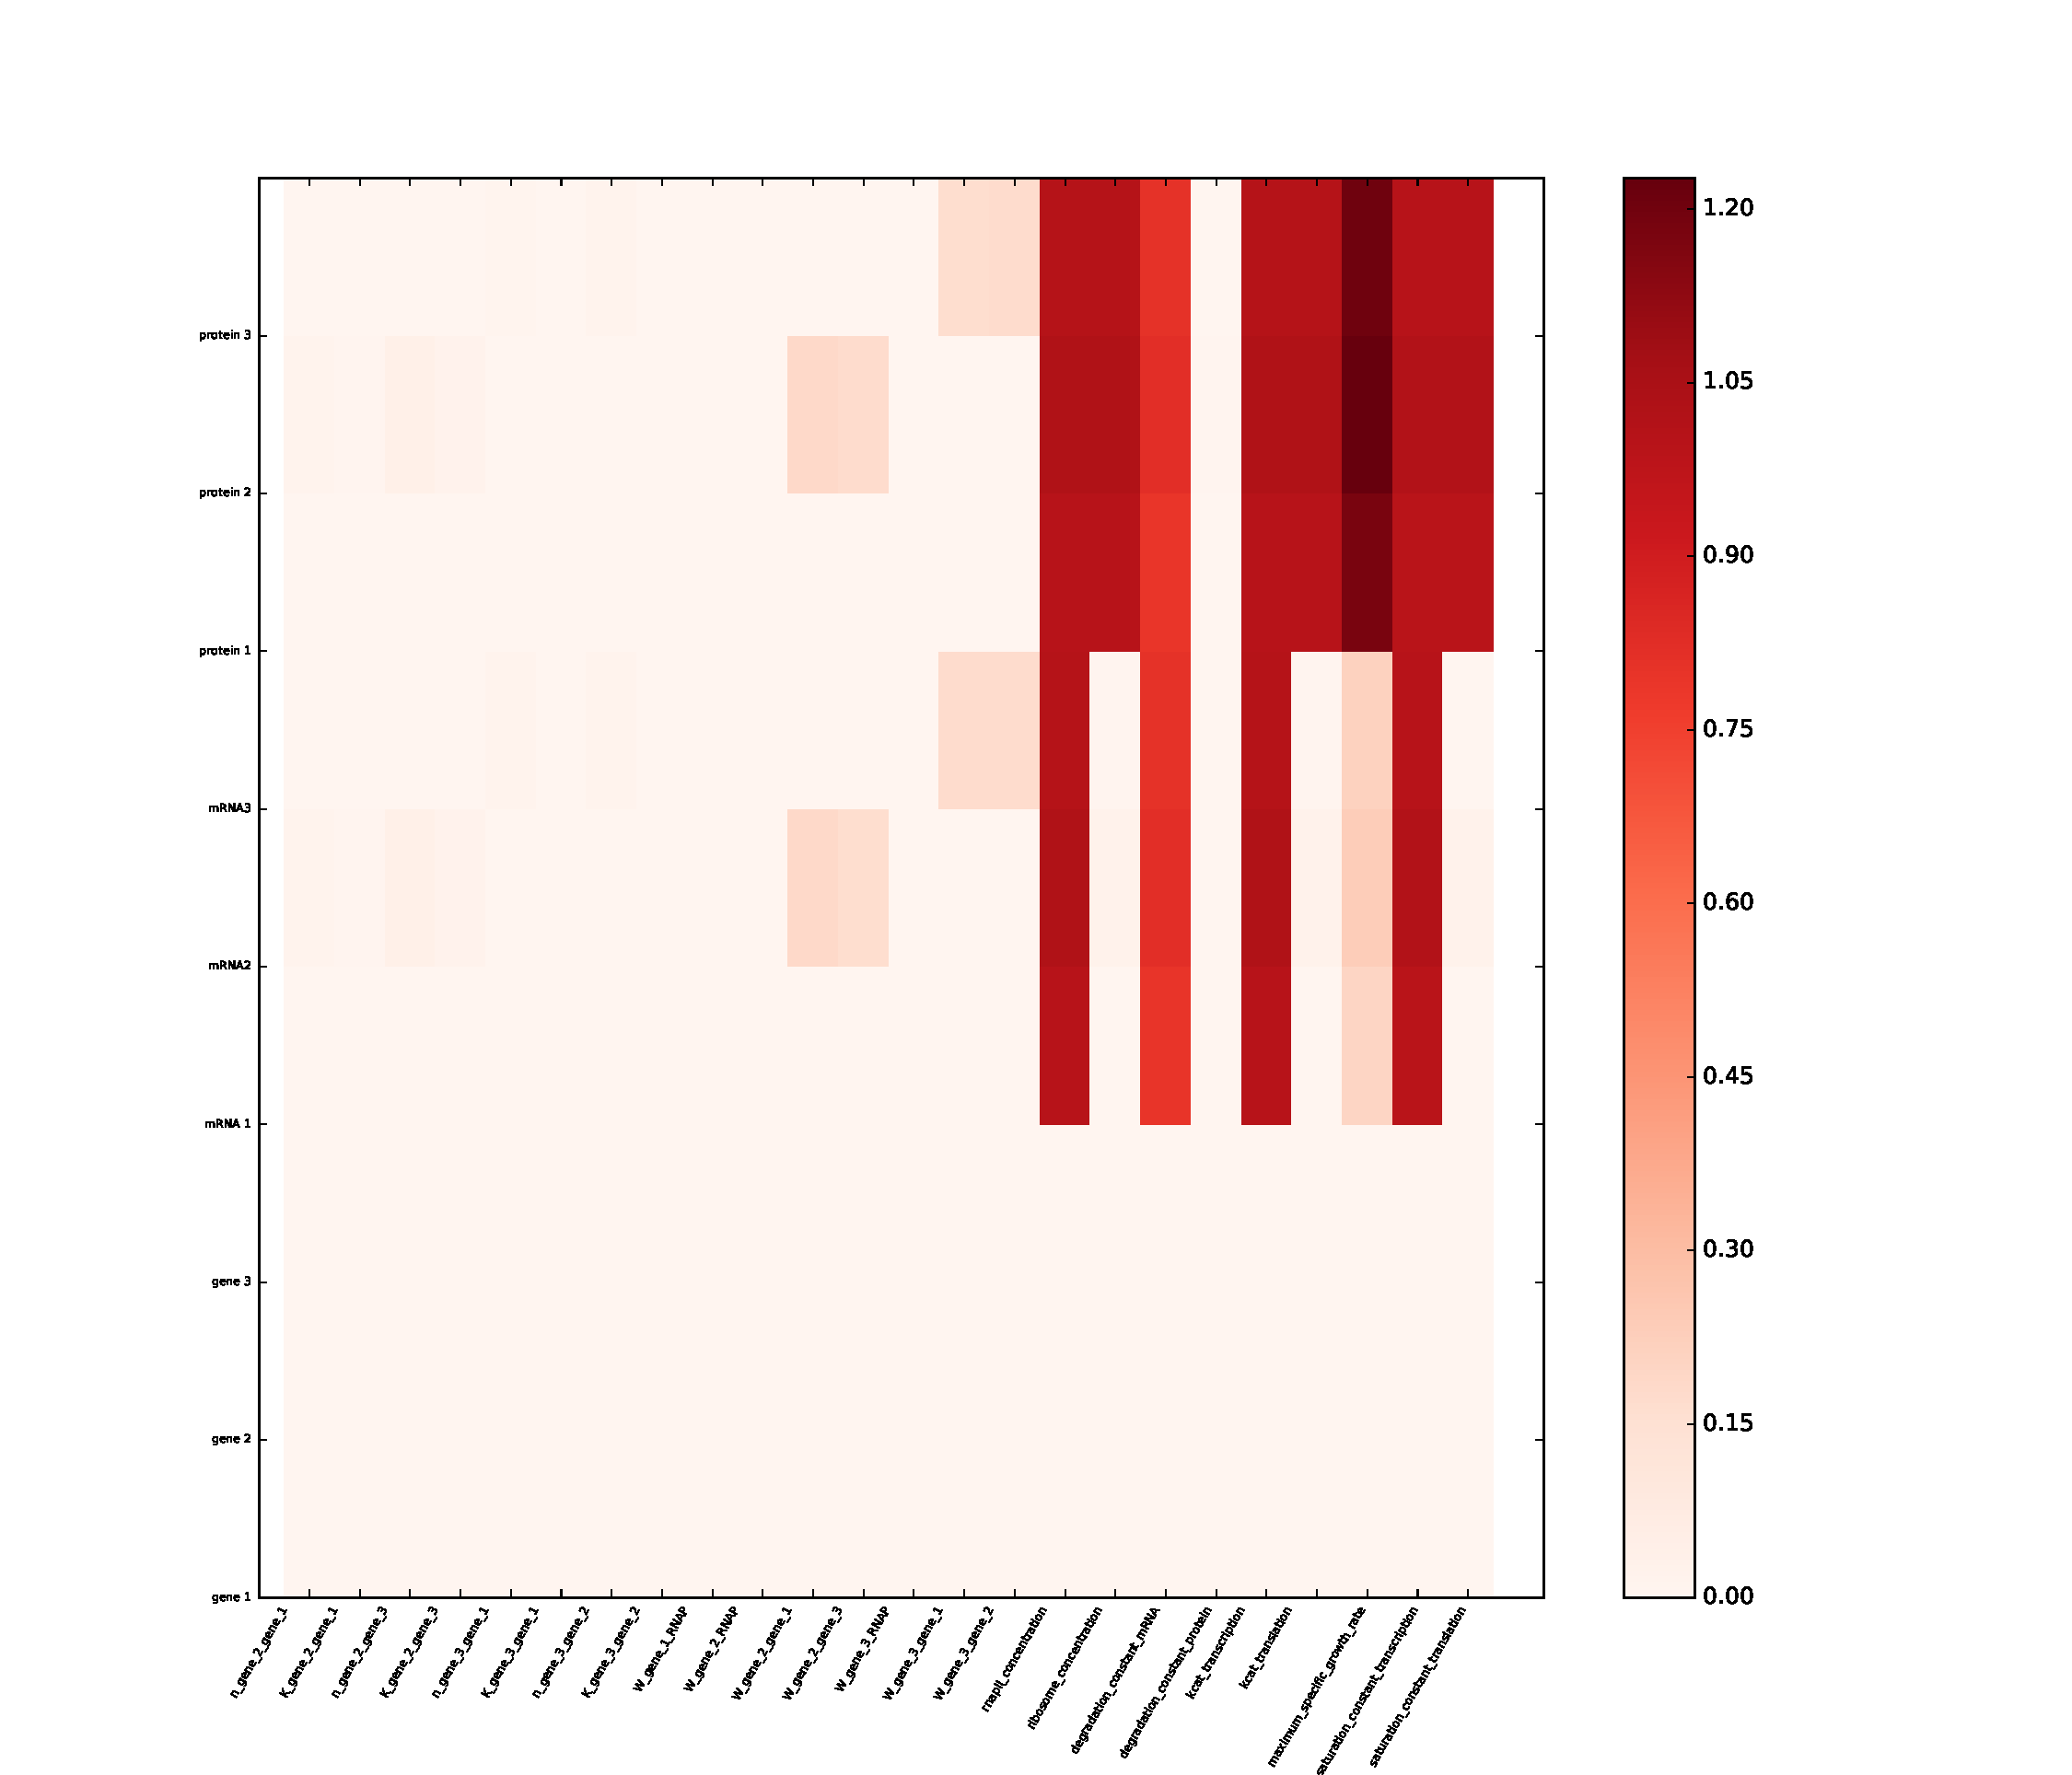
\includegraphics[width=12cm]{../ThreeGeneRachelV2/figures/ParameterSpeciesInteractionsFrom10to70}
\caption{Heat map produced from time averaged sensitivity array of three gene network during induction}
\label{fig:P2Induced}
\end{figure}

As expected, when only the concentrations of P3 and mRNA are measured, the number of measurable species is fewer than in the case when all species are measured, as shown in Figure \ref{fig:P2Freq}. Additionally, as measuring frequency decreases (time between measurements increases), so does the number of estimable parameters. The details of which parameters are estimable at $\epsilon = .001$ are given in the  supplementary material.
\begin{figure}[!htb]
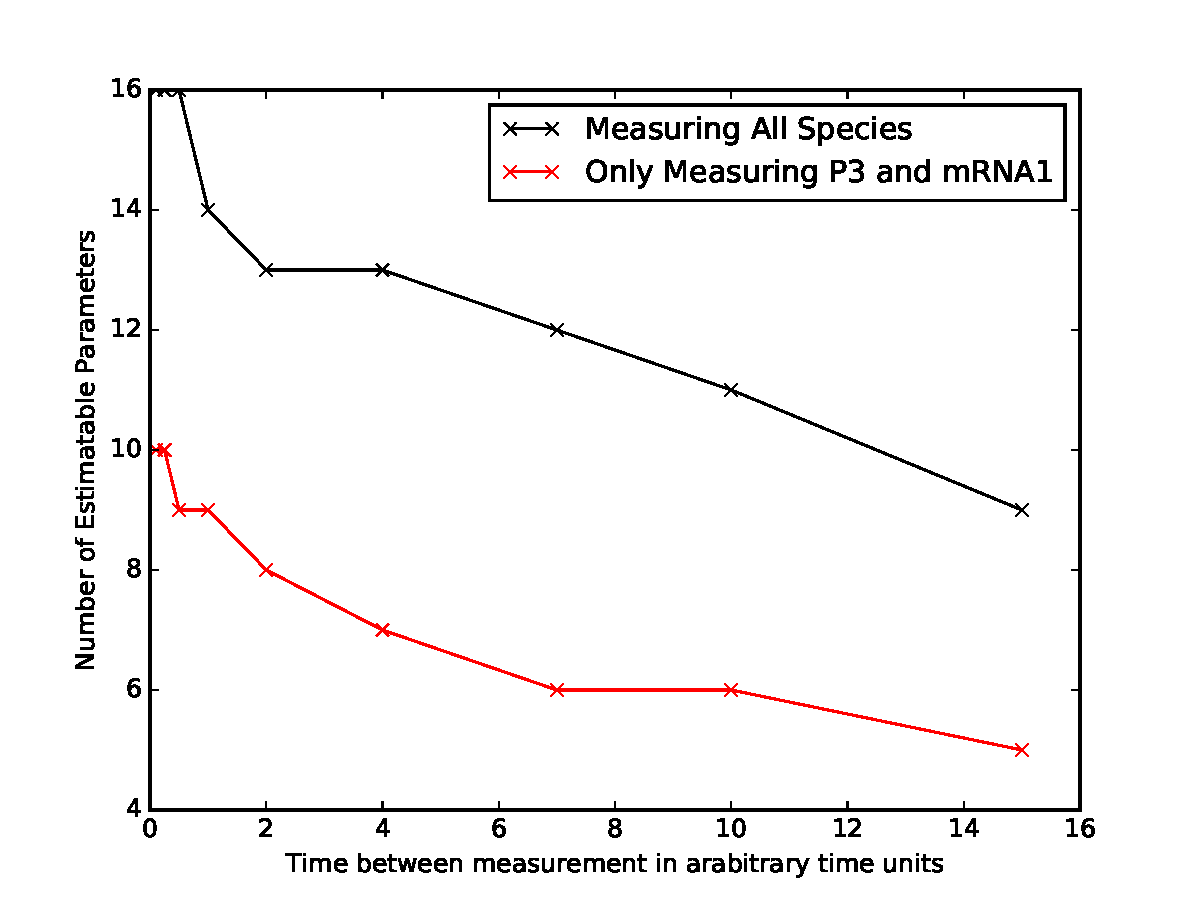
\includegraphics[width=12cm]{../ThreeGeneRachelV2/figures/NumberOfEstamatableParamsAsAFunctionOfFreq}
\caption{Number of estimable parameters at $\epsilon =.001$ as a function of sampling frequency}
\label{fig:P2Freq}
\end{figure}
\newpage
\section*{Problem 3} 
Based on close examination of Figure 2 in the provided problem set, it appears that the levels of P3 and P1 and P2 are inversely related, so that either P1 or P2 represses the production of P3. Since it appears that the level of P1 begins to increase before the level of P2 begins to rise, I hypothesized that the inducer interacts with P1. This leads to network 1:\\

\begin{centering}
\texttt{gene$_1$ induces (gene$_2$)\\
gene$_2$ activates (gene$_1$) \\
gene$_2$ represses (gene$_3$)}\\
\end{centering}

After optimization, this leads to a pretty decent fit of the model data, as shown in Figure \ref{fig:P3Layout1}. I used the Nelder-Mead algorithm as implemented by the NLopt package to perform the optimization, by minimizing the summed mean squared errors between the given protein data and the model prediction, with the bounds set to 100 times the hand fit parameters to 1/100th of the hand fit parameters.
\begin{figure}[!htb]
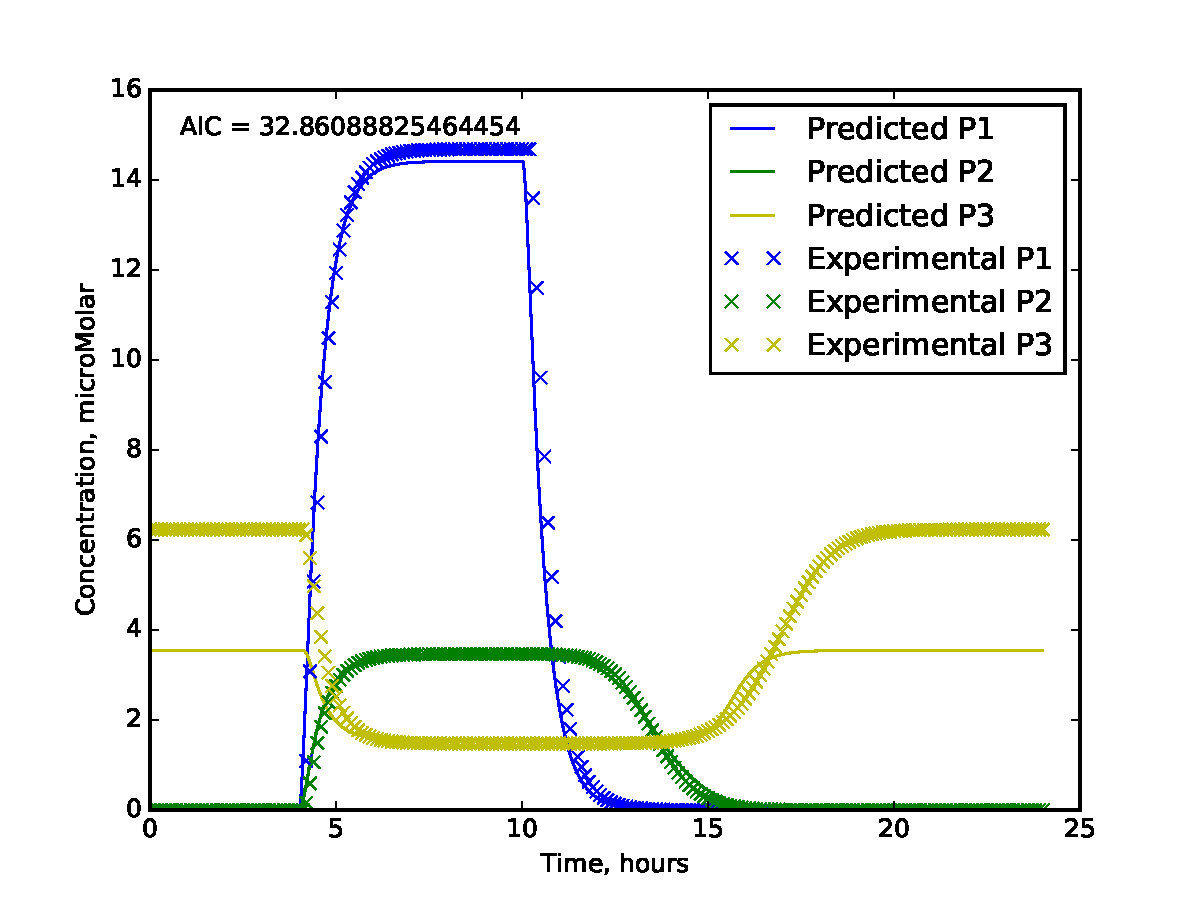
\includegraphics[width=12cm]{../Problem3/figures/postNMPlotLayout1}
\caption{Model performance for network layout 1. Xs represent simulated data, lines represent model predictions.}
\label{fig:P3Layout1}
\end{figure}

Another possibility is that once gene 1 is induced, it activates gene 2 and inhibits gene 3, while protein 2 reduces the production of protein three, as described in network 2:\\

\begin{centering}
\texttt{gene$_1$ induces gene$_2$\\
gene$_1$ represses gene$_3$\\
gene$_2$ represses gene$_3$\\
}
\end{centering}
This model, even after optimization, did not appear to do go as good of a job of capturing the experimental data, as it under-predicts all of the protein concentrations, as shown in Figure \ref{fig:P3Layout3}.
\begin{figure}[!htb]
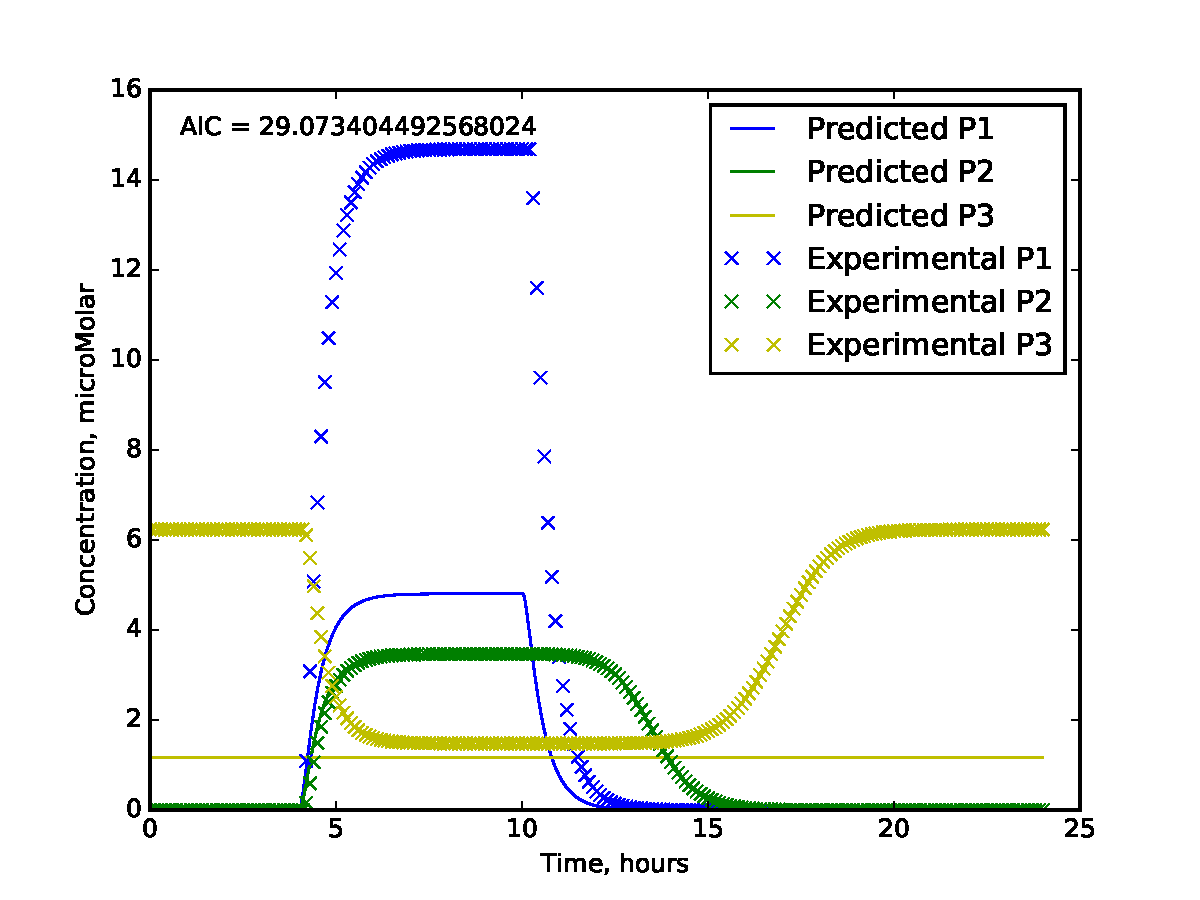
\includegraphics[width=12cm]{../Problem3/figures/postNMPlotLayout3}
\caption{Model performance for network layout 2. Xs represent simulated data, lines represent model predictions.}
\label{fig:P3Layout3}
\end{figure}

However, I opted to carry the analysis further and used the method of Kremling et all to inform my decision about which experiment should be performed to distinguish between the two models. I once again used the Nelder Mead algorithm as implemented by NLopt to maximize $u$, essentially, the difference between the model performance under differing experimental conditions. I allowed the weights of the RNAP on the genes to vary, simulating inducing different genes, as well as the initial concentrations of the genes, simulating knock outs. Following this, it appeared that the most informative experiment to perform was to induce gene 1, which when provided with experimental results supported model structure 1. Even though model 2 has a lower AIC, it completely fails to capture the dynamics of protein 3.

I also decided to compare the case of the feed back loop to having the feed back loop absent. \\

\begin{centering}
\texttt{
gene$_1$ induces (gene$_2$)\\
gene$_2$ represses (gene$_3$)\\
}
\end{centering}

The case with no feedback loop will be named case 5, because the intermediate cases did not prove illuminating. After parameter optimization, this proposed network layout also failed to precisely capture the protein 3 dynamics, but had a low AIC, partially because it contains fewer parameters than models 1 and 2. I figured that the easiest way to differentiate between models 1 and 5 would be to induce gene 2-as if the feedback loop is present, when gene 2 is induced, the concentration of protein 1 will rise, if not, it will remain low. Figure \ref{fig:P3Layout5} shows the performance on this model on the experimental data originally given, and Figure \ref{fig:P3Layout5Induce2} shows its performance when only gene 2 is induced.  
\begin{figure}[!htb]
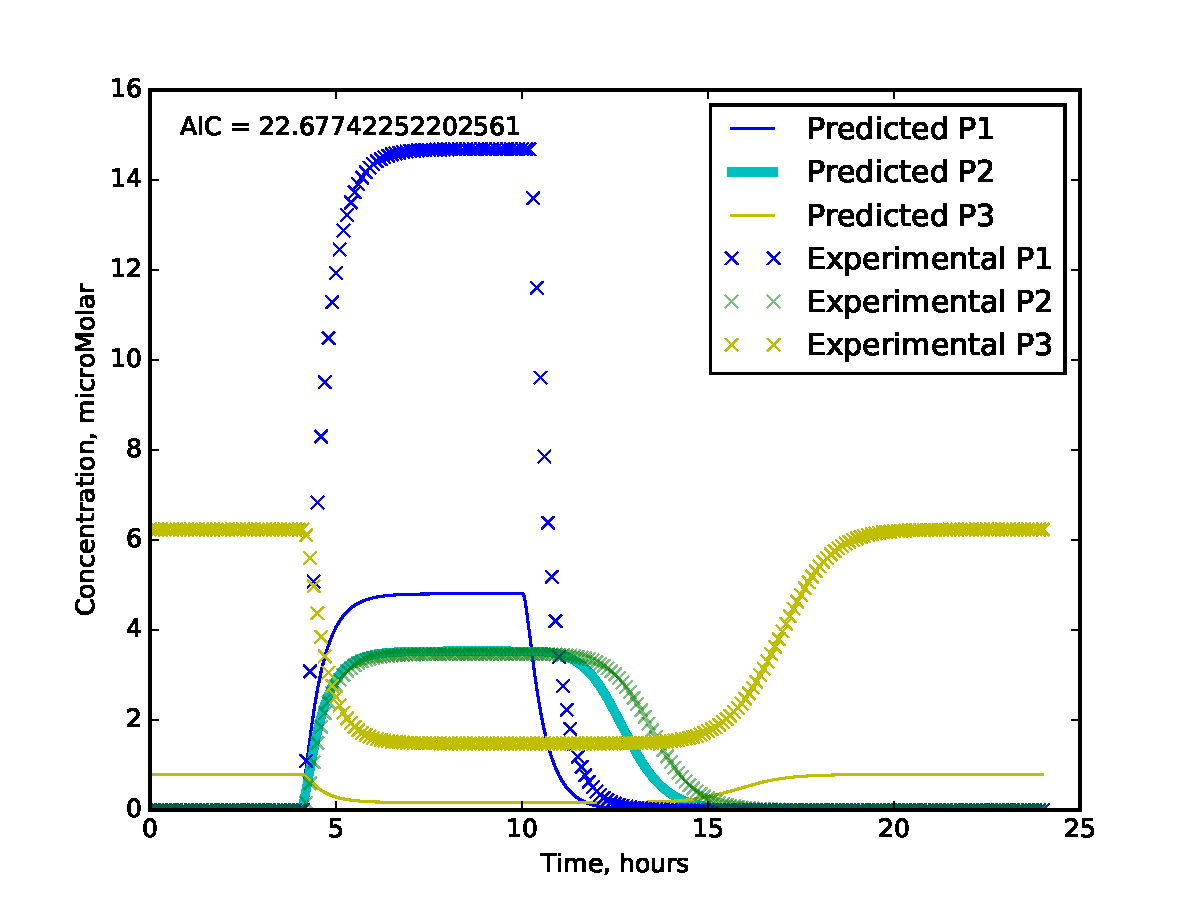
\includegraphics[width=12cm]{../Problem3/figures/postNMPlotLayout5WGene2Info}
\caption{Model performance for network layout 5. Xs represent simulated data, lines represent model predictions. Using parameters generated by fitting on inducing gene 2. While the fit is far from perfect, these parameters do capture the shape of the protein interactions.}
\label{fig:P3Layout5}
\end{figure}

\begin{figure}[!htb]
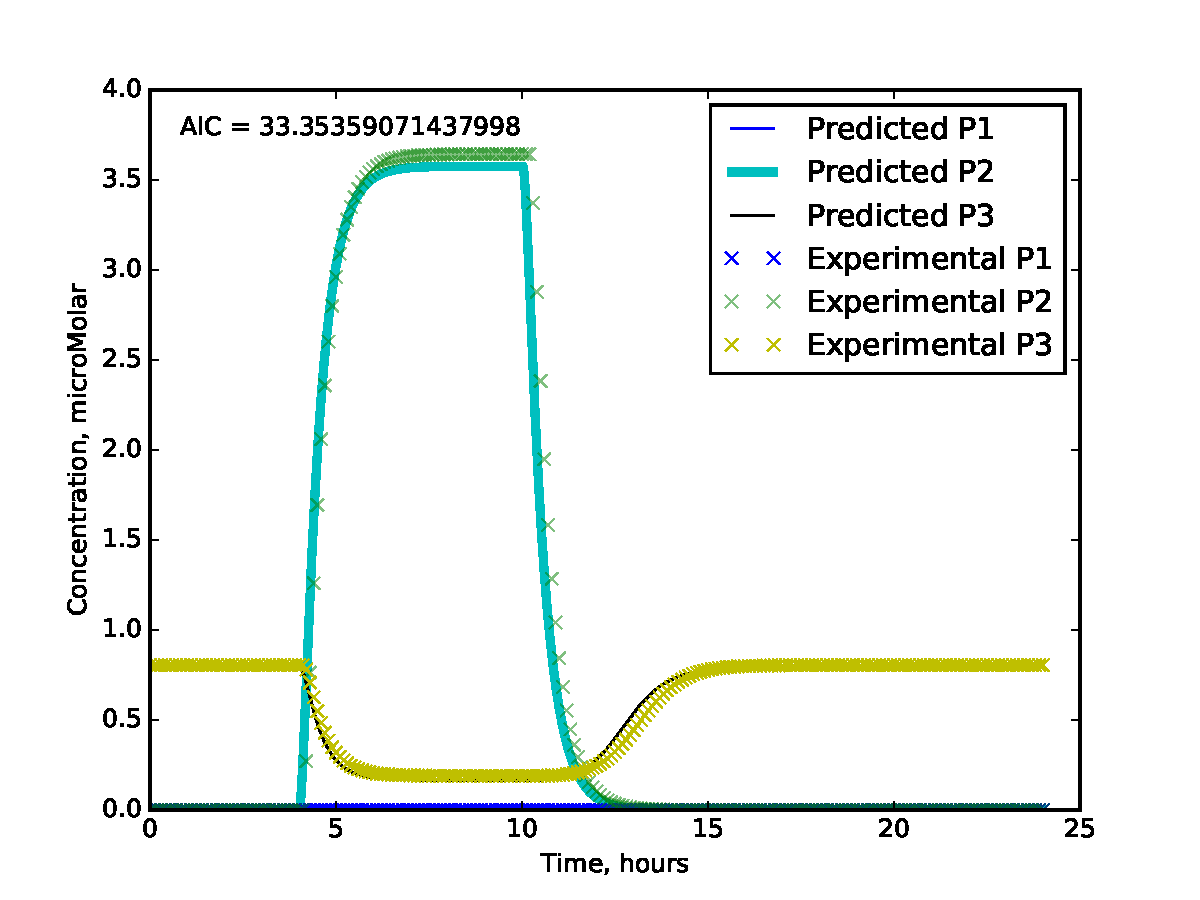
\includegraphics[width=12cm]{../Problem3/figures/postNMPlotLayout5Gene2}
\caption{Model performance for network layout 5 when gene 2 is induced. Xs represent simulated data, lines represent model predictions.}
\label{fig:P3Layout5Induce2}
\end{figure}

Model 5 performs very well in this case, as quantified by the low AIC for both the case of gene 1 and gene 2 being induced, leading me to hypothesize that it is more likely than model 1, as it has a low AIC for the case of inducing gene 1. In conclusion, I believe model 5 is the most probable, followed by model 1, and then 2.

\newpage
\newgeometry{left=.1cm,bottom=0.1cm,right=.1cm,top=.1cm} 
\begin{landscape}
\section*{Supplemental Material}
\subsection*{Details of Estimable Parameters}
%{\fontsize{2}{2}\selectfont
\scalebox{0.5}{
\begin{minipage}{\textwidth}
0.1\\
n\_gene\_2\_gene\_1,K\_gene\_2\_gene\_1,n\_gene\_3\_gene\_1,K\_gene\_3\_gene\_1,W\_gene\_1\_RNAP,W\_gene\_2\_gene\_1,W\_gene\_2\_gene\_3,W\_gene\_3\_gene\_1,W\_gene\_3\_gene\_2,rnapII\_concentration,ribosome\_concentration,degradation\_constant\_mRNA,kcat\_transcription,kcat\_translation,maximum\_specific\_growth\_rate,saturation\_constant\_translation\\
n\_gene\_3\_gene\_1,K\_gene\_3\_gene\_1,W\_gene\_1\_RNAP,W\_gene\_3\_gene\_1,W\_gene\_3\_gene\_2,rnapII\_concentration,degradation\_constant\_mRNA,kcat\_transcription,kcat\_translation,maximum\_specific\_growth\_rate\\
0.25\\
n\_gene\_2\_gene\_1,K\_gene\_2\_gene\_1,n\_gene\_3\_gene\_1,K\_gene\_3\_gene\_1,W\_gene\_1\_RNAP,W\_gene\_2\_gene\_1,W\_gene\_2\_gene\_3,W\_gene\_3\_gene\_1,W\_gene\_3\_gene\_2,rnapII\_concentration,ribosome\_concentration,degradation\_constant\_mRNA,kcat\_transcription,kcat\_translation,maximum\_specific\_growth\_rate,saturation\_constant\_translation\\
n\_gene\_3\_gene\_1,K\_gene\_3\_gene\_1,W\_gene\_1\_RNAP,W\_gene\_3\_gene\_1,W\_gene\_3\_gene\_2,rnapII\_concentration,degradation\_constant\_mRNA,kcat\_transcription,kcat\_translation,maximum\_specific\_growth\_rate\\
0.5\\
n\_gene\_2\_gene\_1,K\_gene\_2\_gene\_1,n\_gene\_3\_gene\_1,K\_gene\_3\_gene\_1,W\_gene\_1\_RNAP,W\_gene\_2\_gene\_1,W\_gene\_2\_gene\_3,W\_gene\_3\_gene\_1,W\_gene\_3\_gene\_2,rnapII\_concentration,ribosome\_concentration,degradation\_constant\_mRNA,kcat\_transcription,kcat\_translation,maximum\_specific\_growth\_rate,saturation\_constant\_translation\\
n\_gene\_3\_gene\_1,K\_gene\_3\_gene\_1,W\_gene\_1\_RNAP,W\_gene\_3\_gene\_2,rnapII\_concentration,degradation\_constant\_mRNA,kcat\_transcription,kcat\_translation,maximum\_specific\_growth\_rate\\
1.0\\
n\_gene\_2\_gene\_1,n\_gene\_3\_gene\_1,W\_gene\_1\_RNAP,W\_gene\_2\_gene\_1,W\_gene\_2\_gene\_3,W\_gene\_3\_gene\_1,W\_gene\_3\_gene\_2,rnapII\_concentration,ribosome\_concentration,degradation\_constant\_mRNA,kcat\_transcription,kcat\_translation,maximum\_specific\_growth\_rate,saturation\_constant\_translation\\
n\_gene\_3\_gene\_1,K\_gene\_3\_gene\_1,W\_gene\_1\_RNAP,W\_gene\_3\_gene\_2,rnapII\_concentration,degradation\_constant\_mRNA,kcat\_transcription,kcat\_translation,maximum\_specific\_growth\_rate\\
2.0\\
n\_gene\_2\_gene\_1,n\_gene\_3\_gene\_1,W\_gene\_1\_RNAP,W\_gene\_2\_gene\_1,W\_gene\_2\_gene\_3,W\_gene\_3\_gene\_1,W\_gene\_3\_gene\_2,rnapII\_concentration,ribosome\_concentration,degradation\_constant\_mRNA,kcat\_transcription,kcat\_translation,maximum\_specific\_growth\_rate\\
n\_gene\_3\_gene\_1,K\_gene\_3\_gene\_1,W\_gene\_1\_RNAP,W\_gene\_3\_gene\_2,rnapII\_concentration,degradation\_constant\_mRNA,kcat\_translation,maximum\_specific\_growth\_rate\\
4.0\\
n\_gene\_2\_gene\_1,n\_gene\_3\_gene\_1,W\_gene\_1\_RNAP,W\_gene\_2\_gene\_1,W\_gene\_2\_gene\_3,W\_gene\_3\_gene\_1,W\_gene\_3\_gene\_2,rnapII\_concentration,ribosome\_concentration,degradation\_constant\_mRNA,kcat\_transcription,kcat\_translation,maximum\_specific\_growth\_rate\\
n\_gene\_3\_gene\_1,W\_gene\_1\_RNAP,W\_gene\_3\_gene\_2,rnapII\_concentration,degradation\_constant\_mRNA,kcat\_translation,maximum\_specific\_growth\_rate\\
7.0\\
n\_gene\_2\_gene\_1,n\_gene\_3\_gene\_1,W\_gene\_1\_RNAP,W\_gene\_2\_gene\_1,W\_gene\_2\_gene\_3,W\_gene\_3\_gene\_1,W\_gene\_3\_gene\_2,rnapII\_concentration,ribosome\_concentration,degradation\_constant\_mRNA,kcat\_translation,maximum\_specific\_growth\_rate\\
n\_gene\_3\_gene\_1,W\_gene\_1\_RNAP,W\_gene\_3\_gene\_2,rnapII\_concentration,degradation\_constant\_mRNA,kcat\_translation\\
10.0\\
n\_gene\_2\_gene\_1,n\_gene\_3\_gene\_1,W\_gene\_1\_RNAP,W\_gene\_2\_gene\_1,W\_gene\_2\_gene\_3,W\_gene\_3\_gene\_1,W\_gene\_3\_gene\_2,rnapII\_concentration,degradation\_constant\_mRNA,kcat\_translation,maximum\_specific\_growth\_rate\\
n\_gene\_3\_gene\_1,W\_gene\_1\_RNAP,W\_gene\_3\_gene\_2,rnapII\_concentration,degradation\_constant\_mRNA,kcat\_translation\\
15.0\\
W\_gene\_2\_gene\_1,W\_gene\_2\_gene\_3,W\_gene\_3\_gene\_1,W\_gene\_3\_gene\_2,rnapII\_concentration,degradation\_constant\_mRNA,kcat\_translation,maximum\_specific\_growth\_rate,saturation\_constant\_translation\\ 
W\_gene\_3\_gene\_2,rnapII\_concentration,degradation\_constant\_mRNA,kcat\_translation,maximum\_specific\_growth\_rate\\ 



\end{minipage}
}\\
First line gives measuring all species, second line is with selected species.
\end{landscape}
\newpage
\subsection*{P2 Species-Species and Parameter Parameter
 Interactions}
 \begin{figure}[!htb]
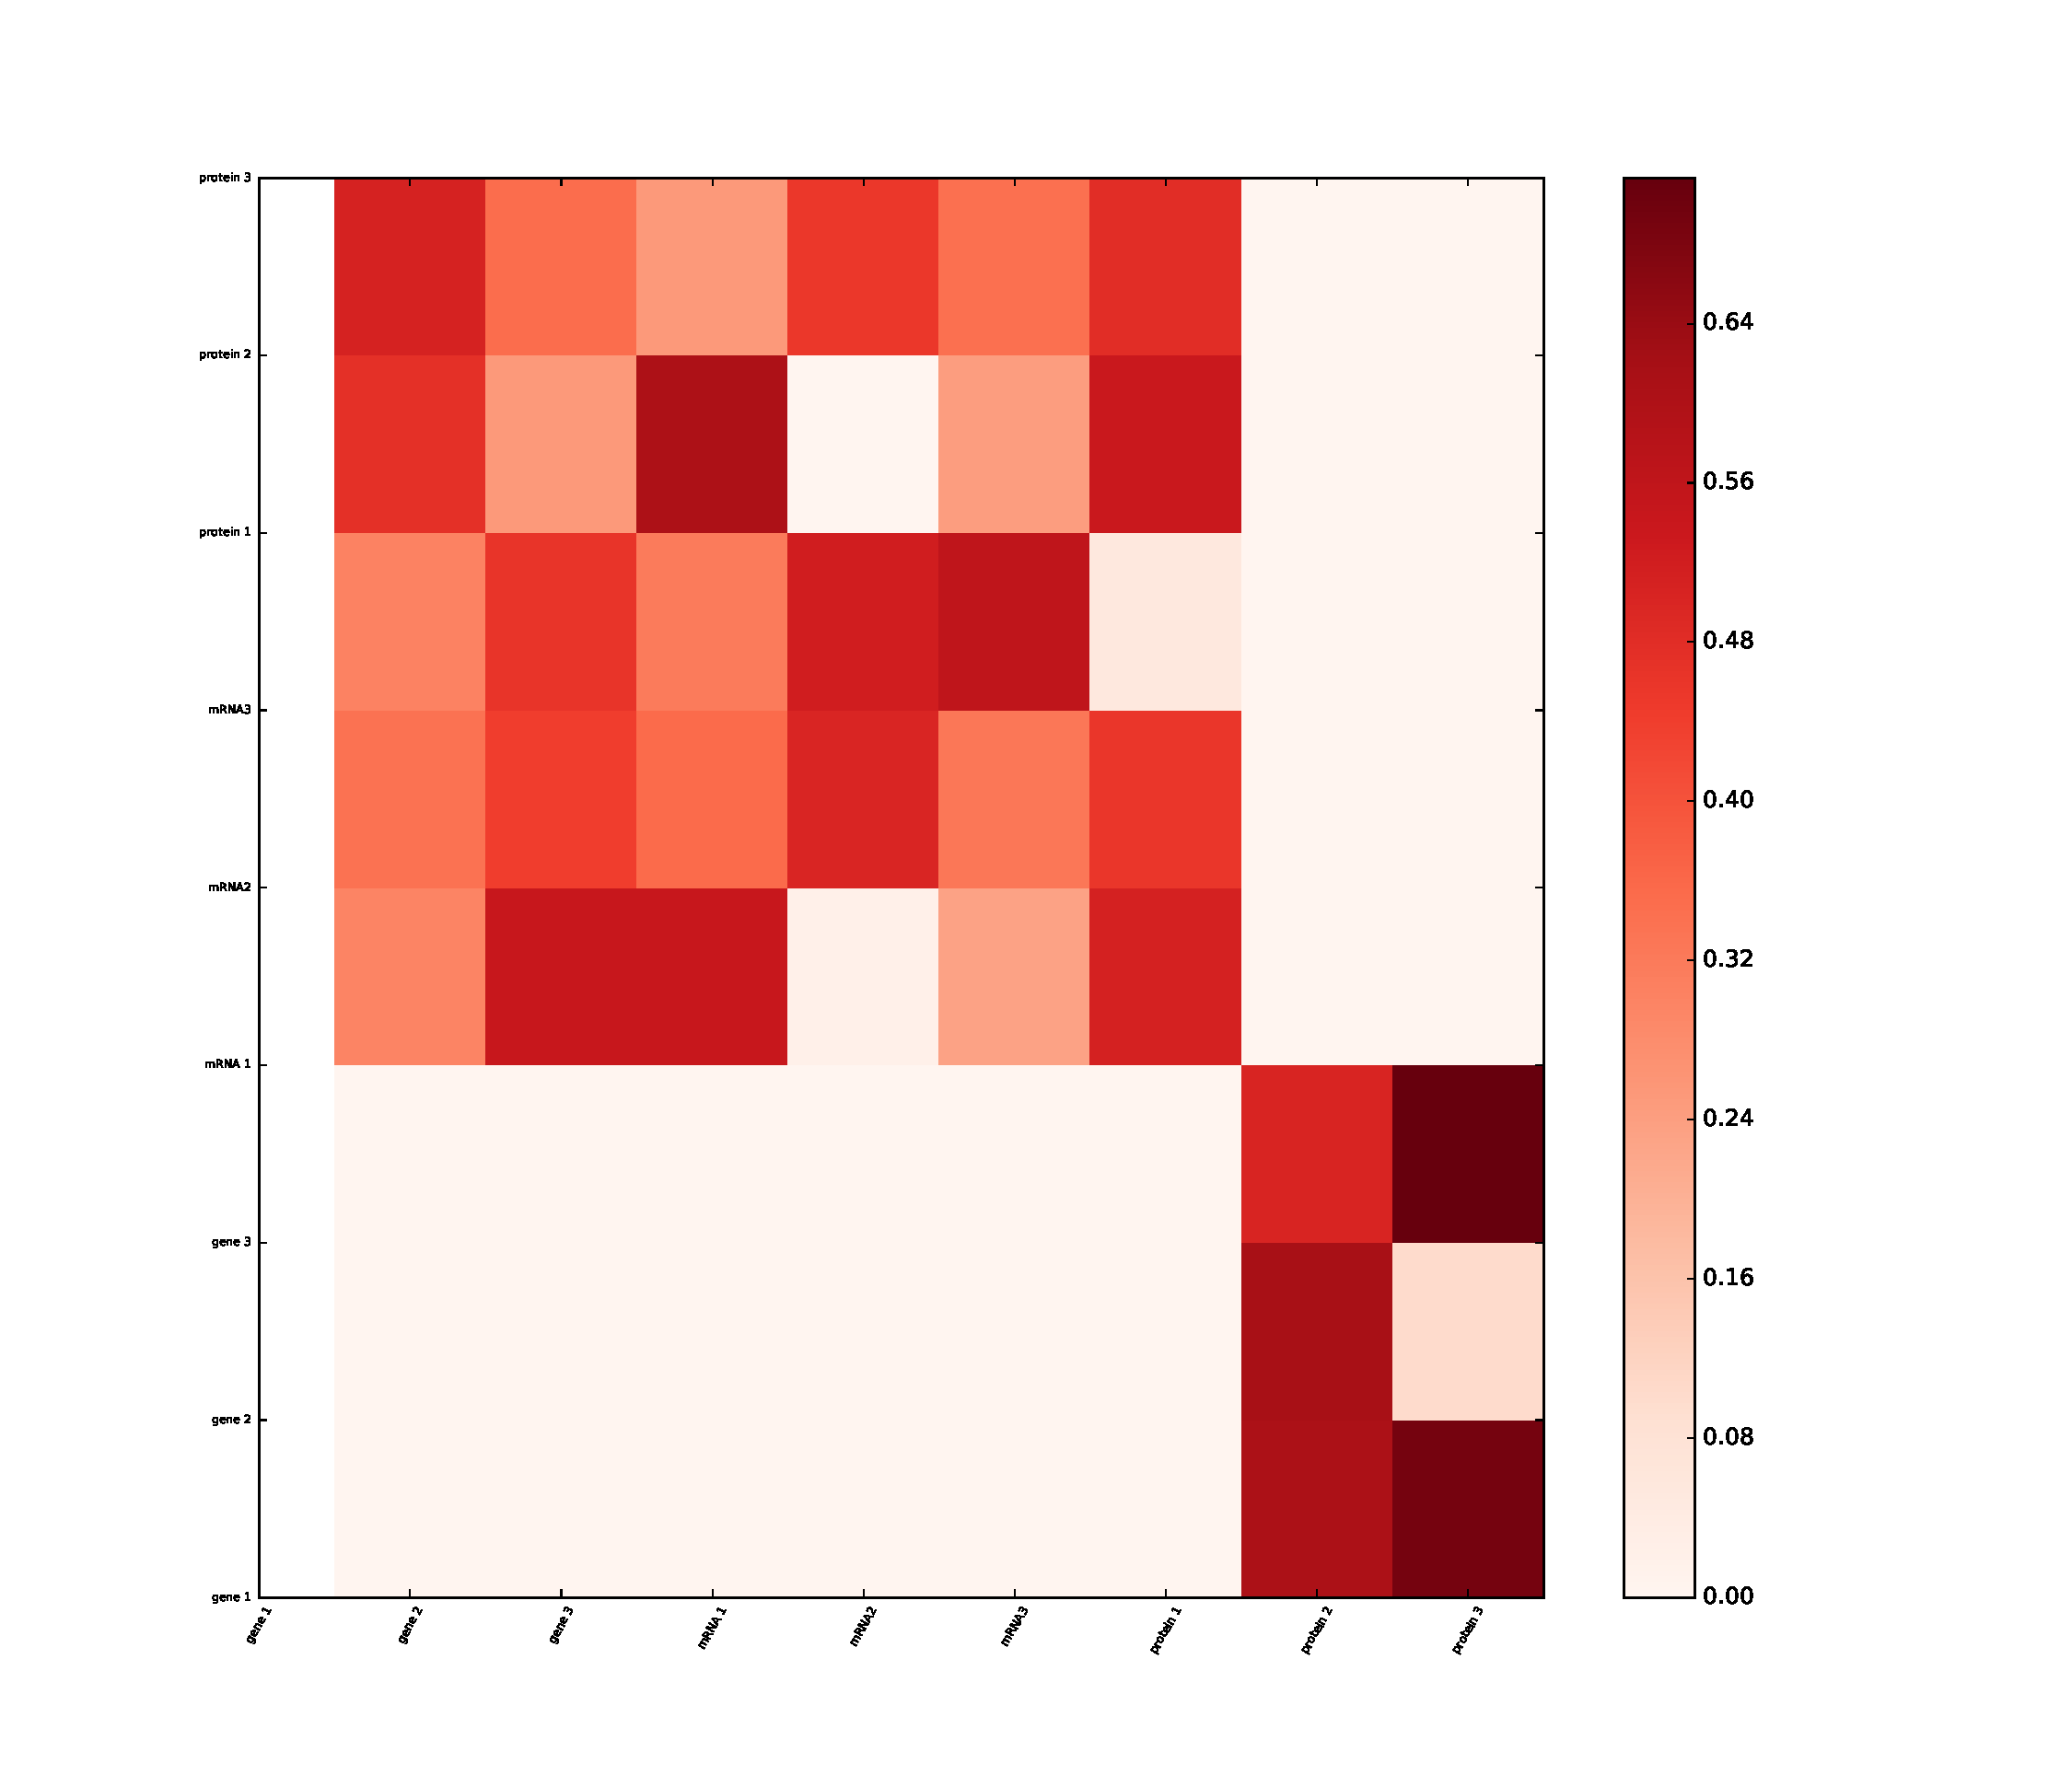
\includegraphics[width=12cm]{../ThreeGeneRachelV2/figures/ProteinInteractionsFrom0to10}
\caption{Heat map produced SVD of time averaged sensitivity of three gene network at steady state showing protein-protein interactions}
\end{figure}

\begin{figure}[!htb]
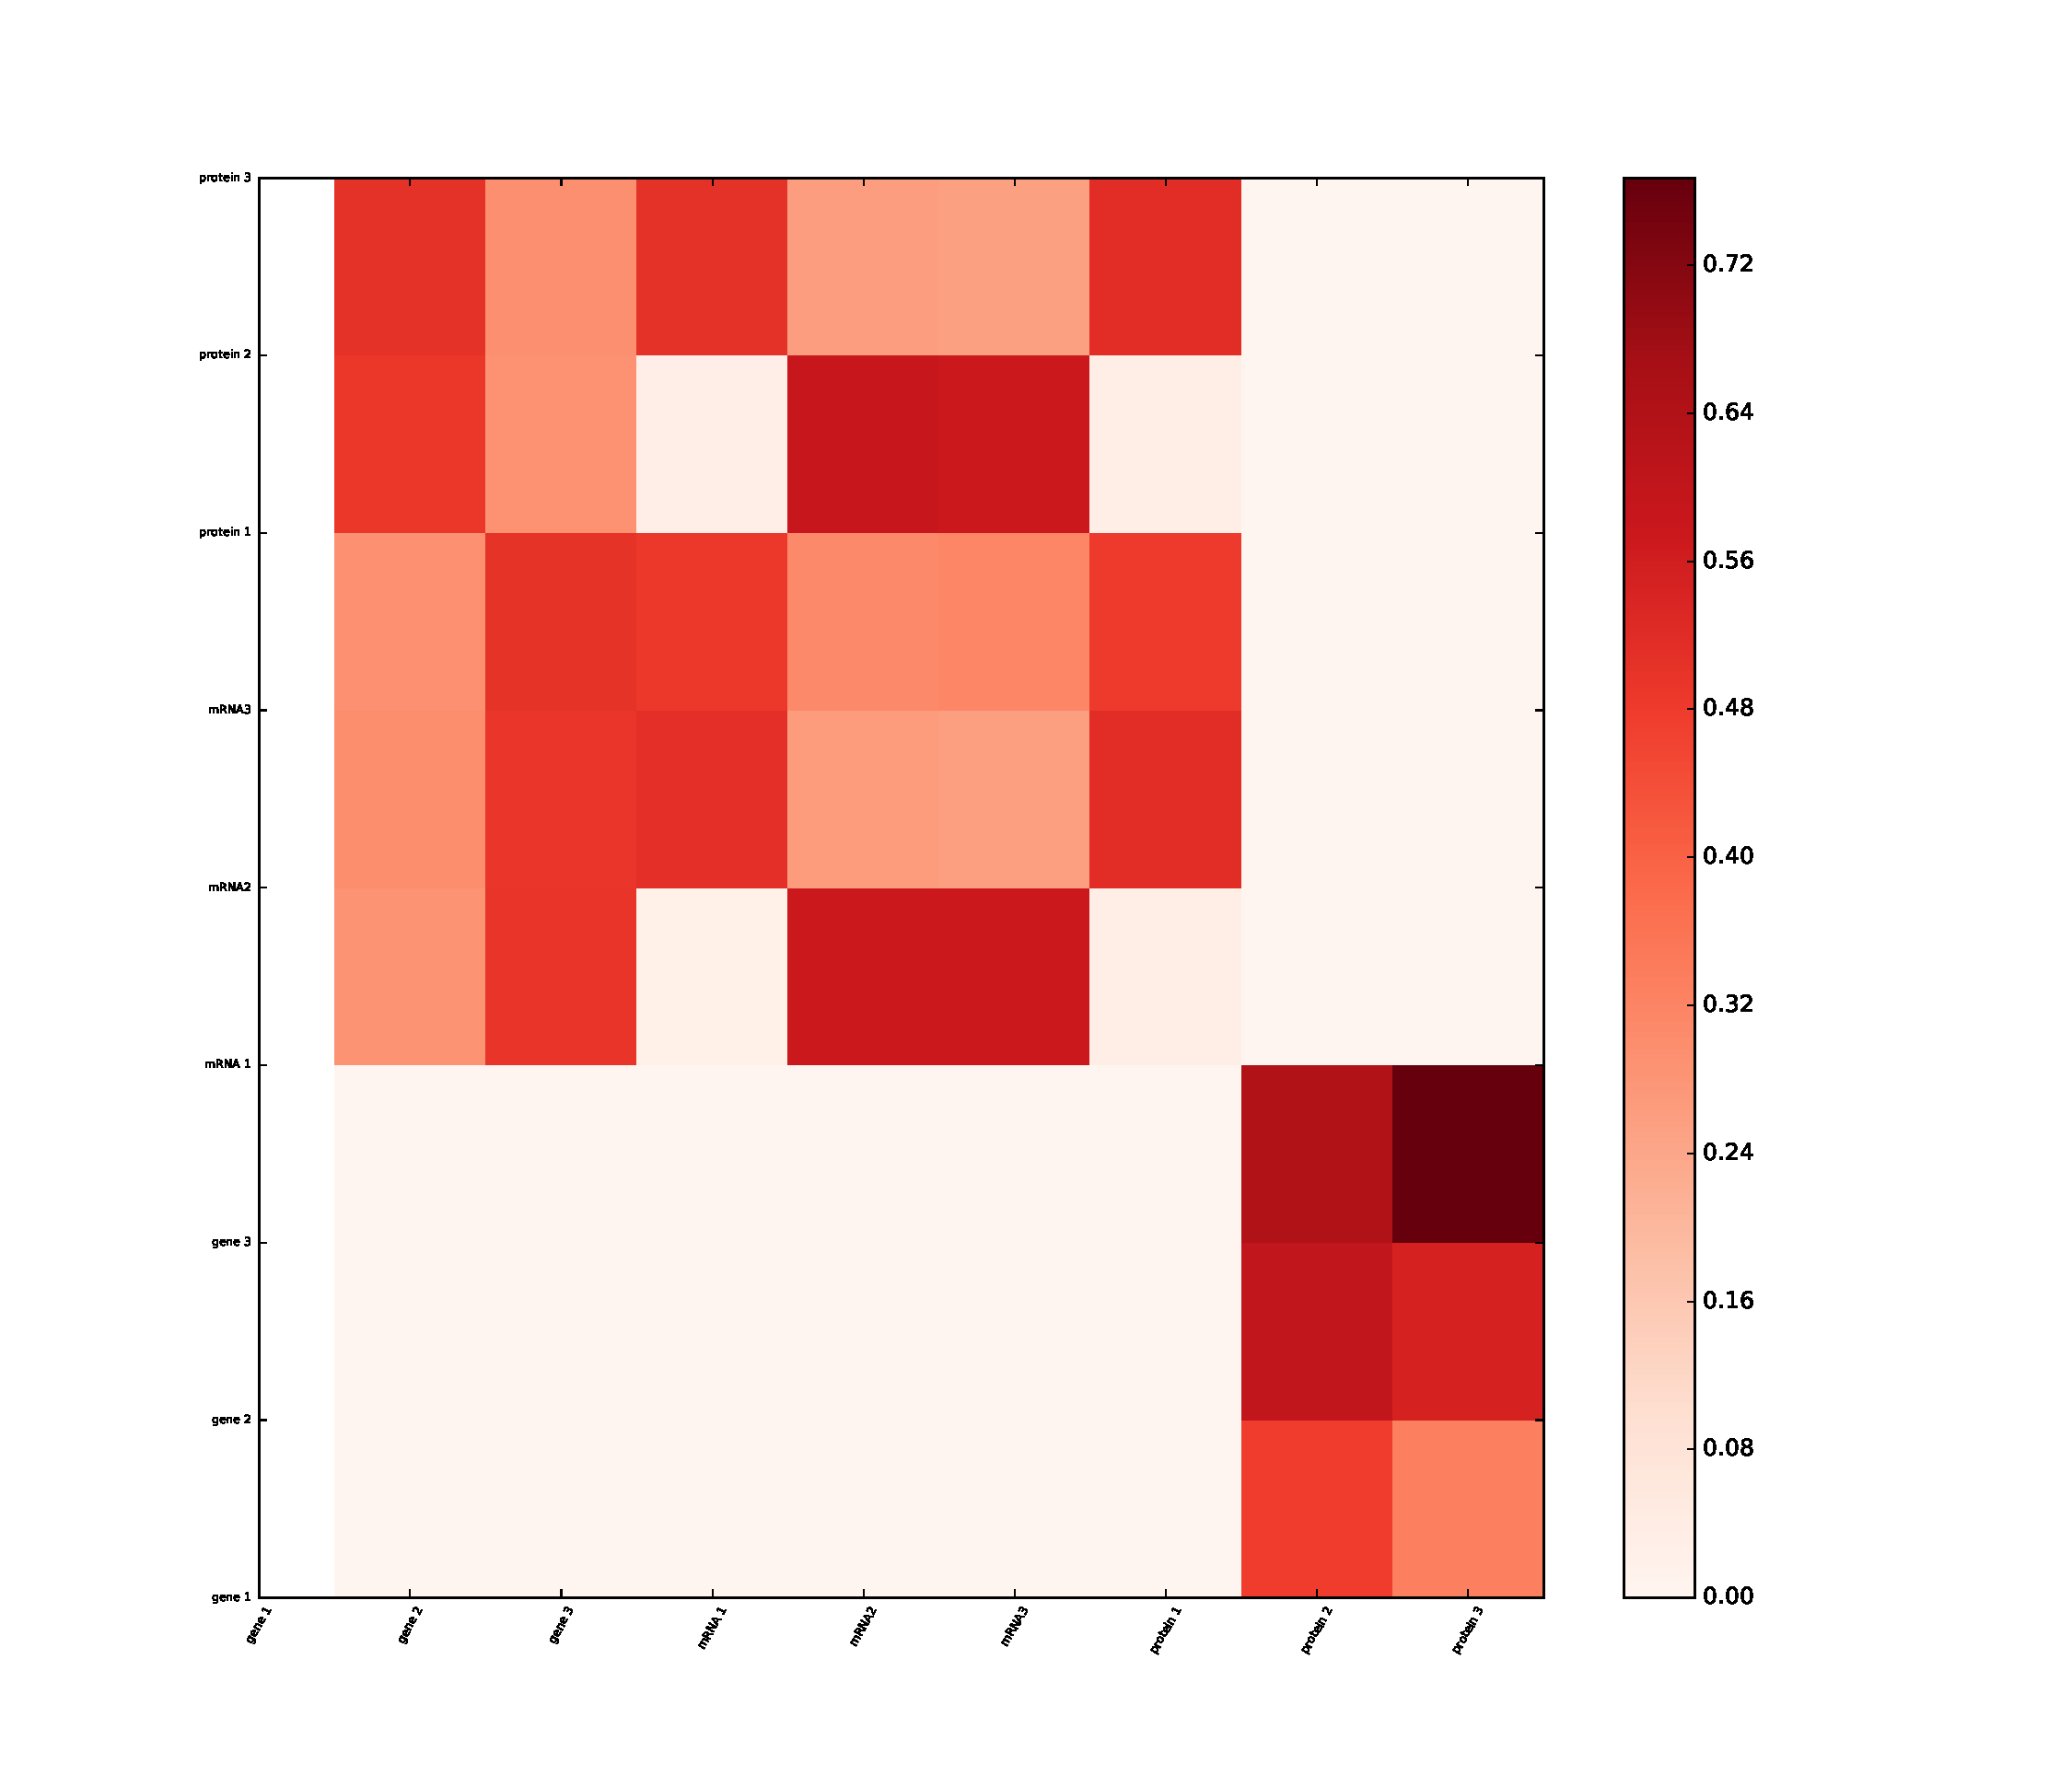
\includegraphics[width=12cm]{../ThreeGeneRachelV2/figures/ProteinInteractionsFrom10to70}
\caption{Heat map produced SVD of time averaged sensitivity of three gene network during induction showing protein-protein interactions}
\end{figure}

 \begin{figure}[!htb]
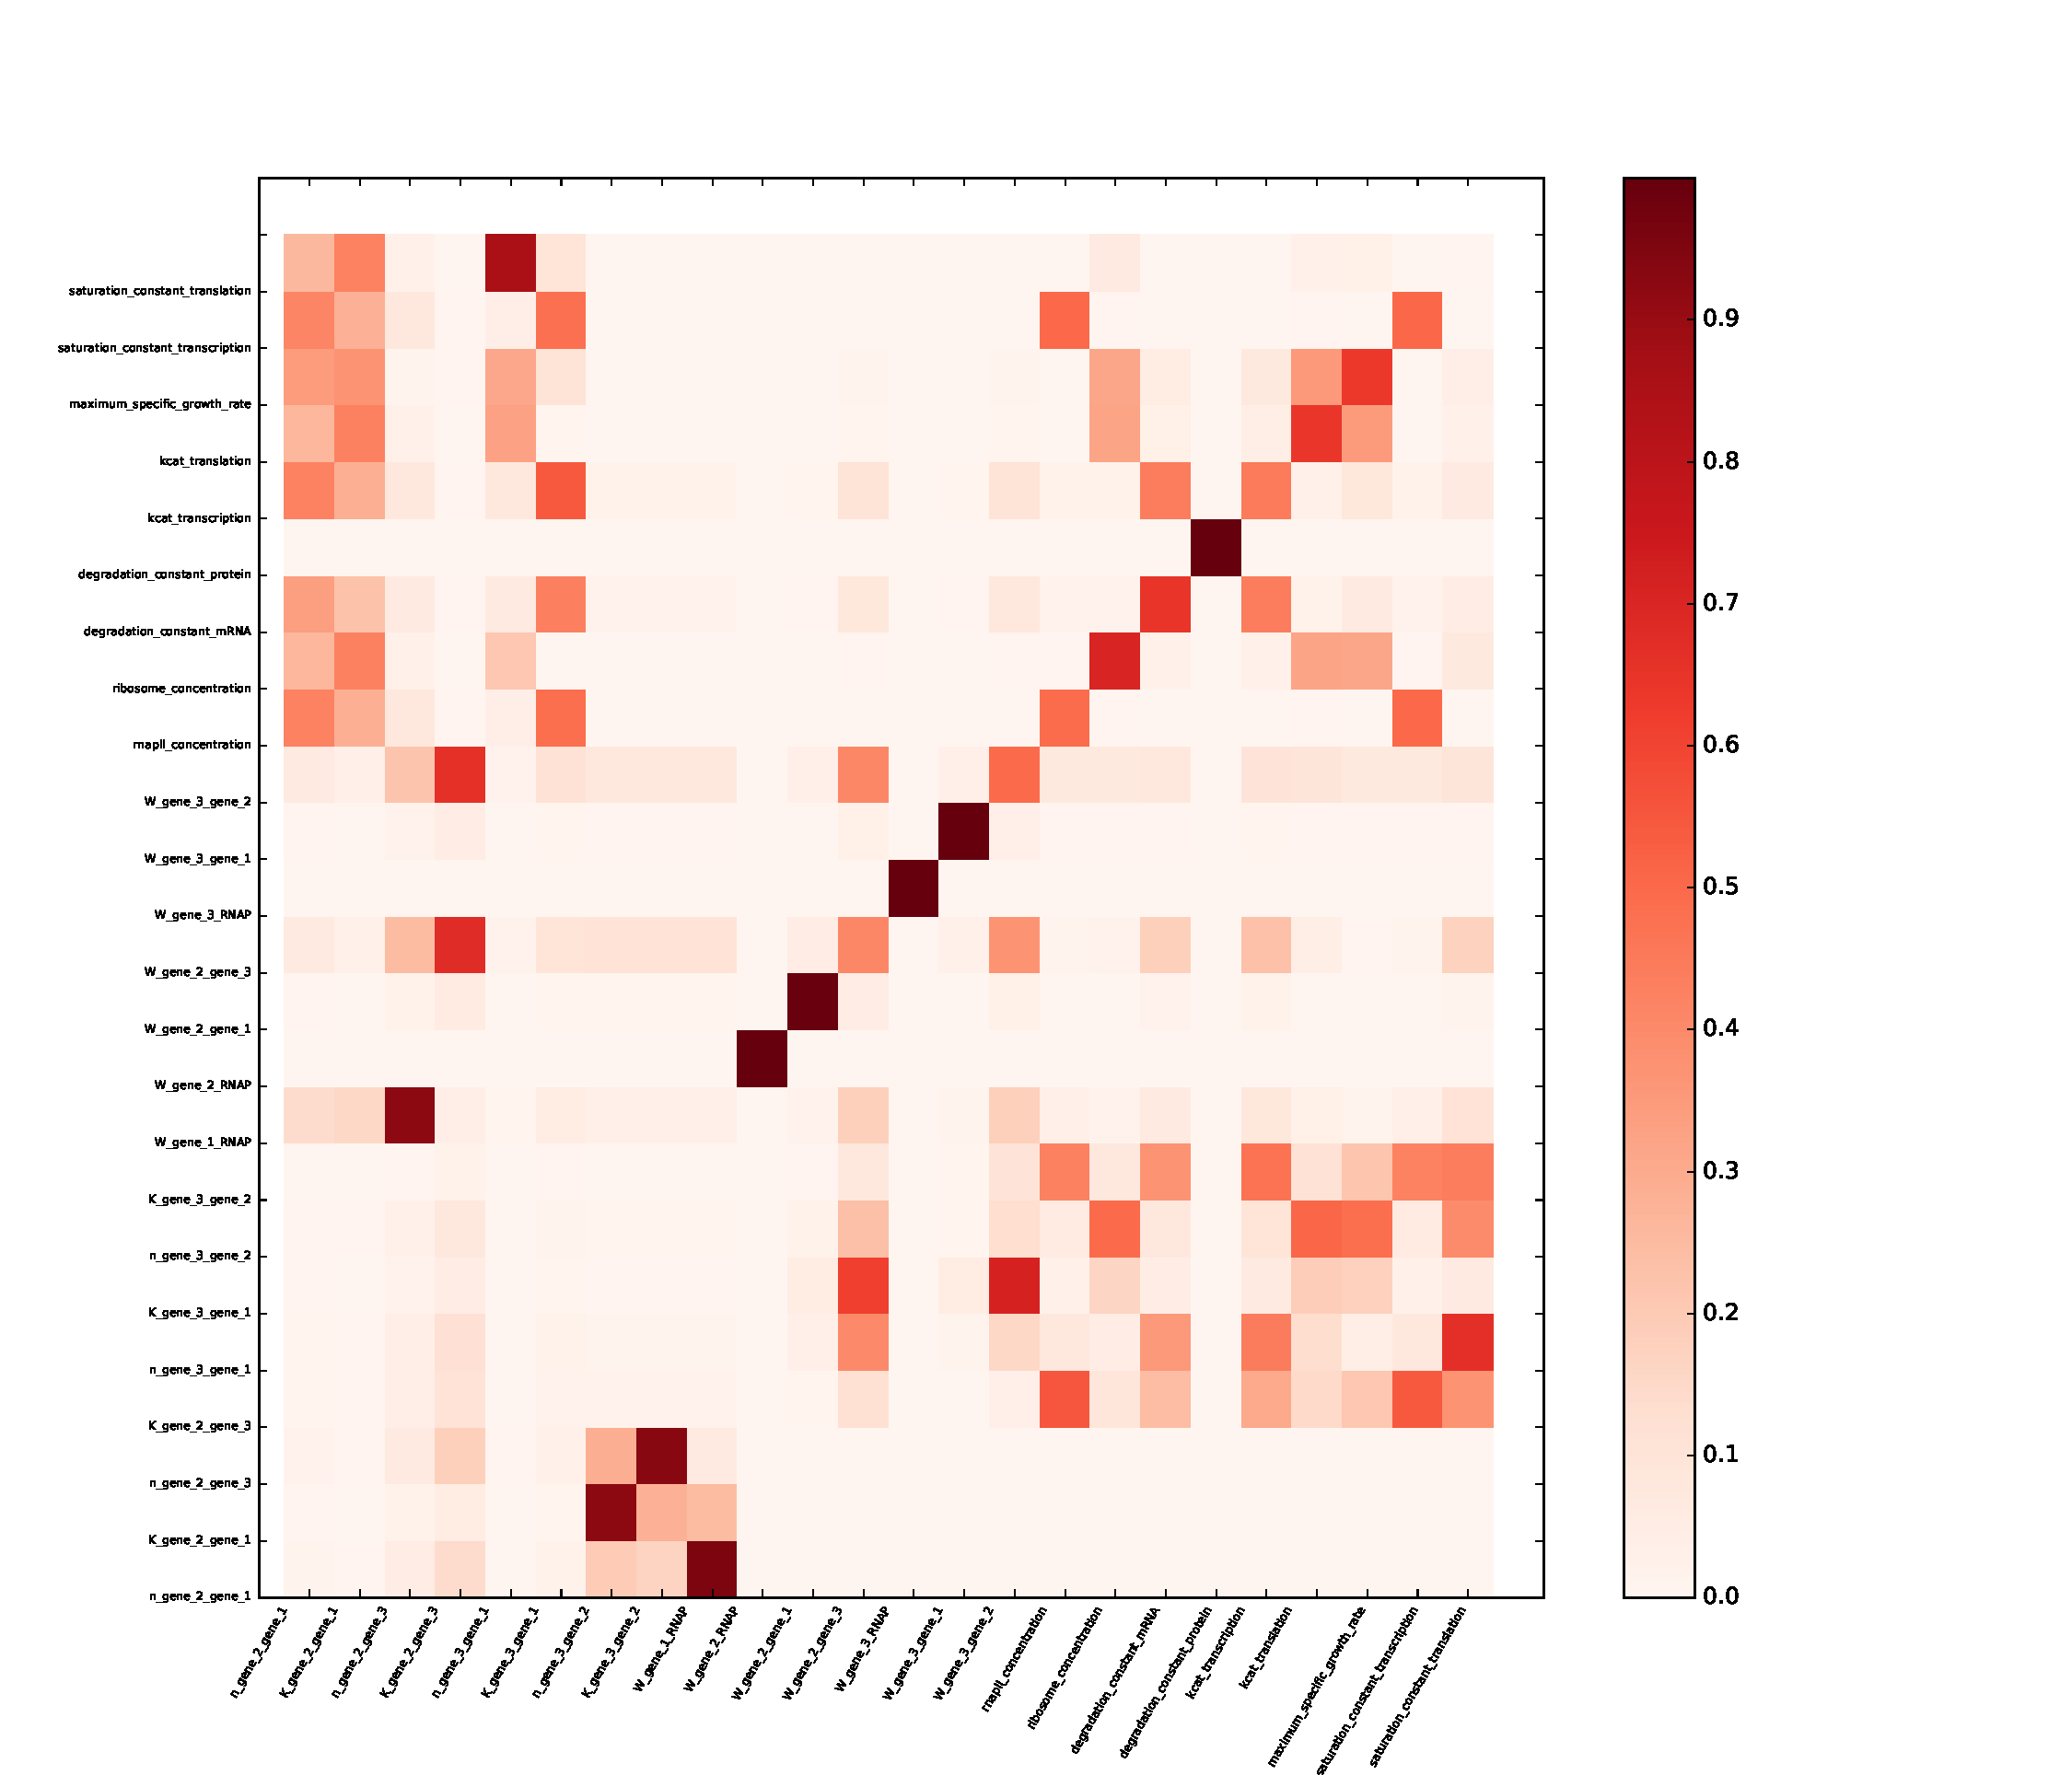
\includegraphics[width=12cm]{../ThreeGeneRachelV2/figures/ParameterInteractionsFrom0to10}
\caption{Heat map produced SVD of time averaged sensitivity of three gene network at steady state showing parameter-parameter interactions}
\end{figure}

\begin{figure}[!htb]
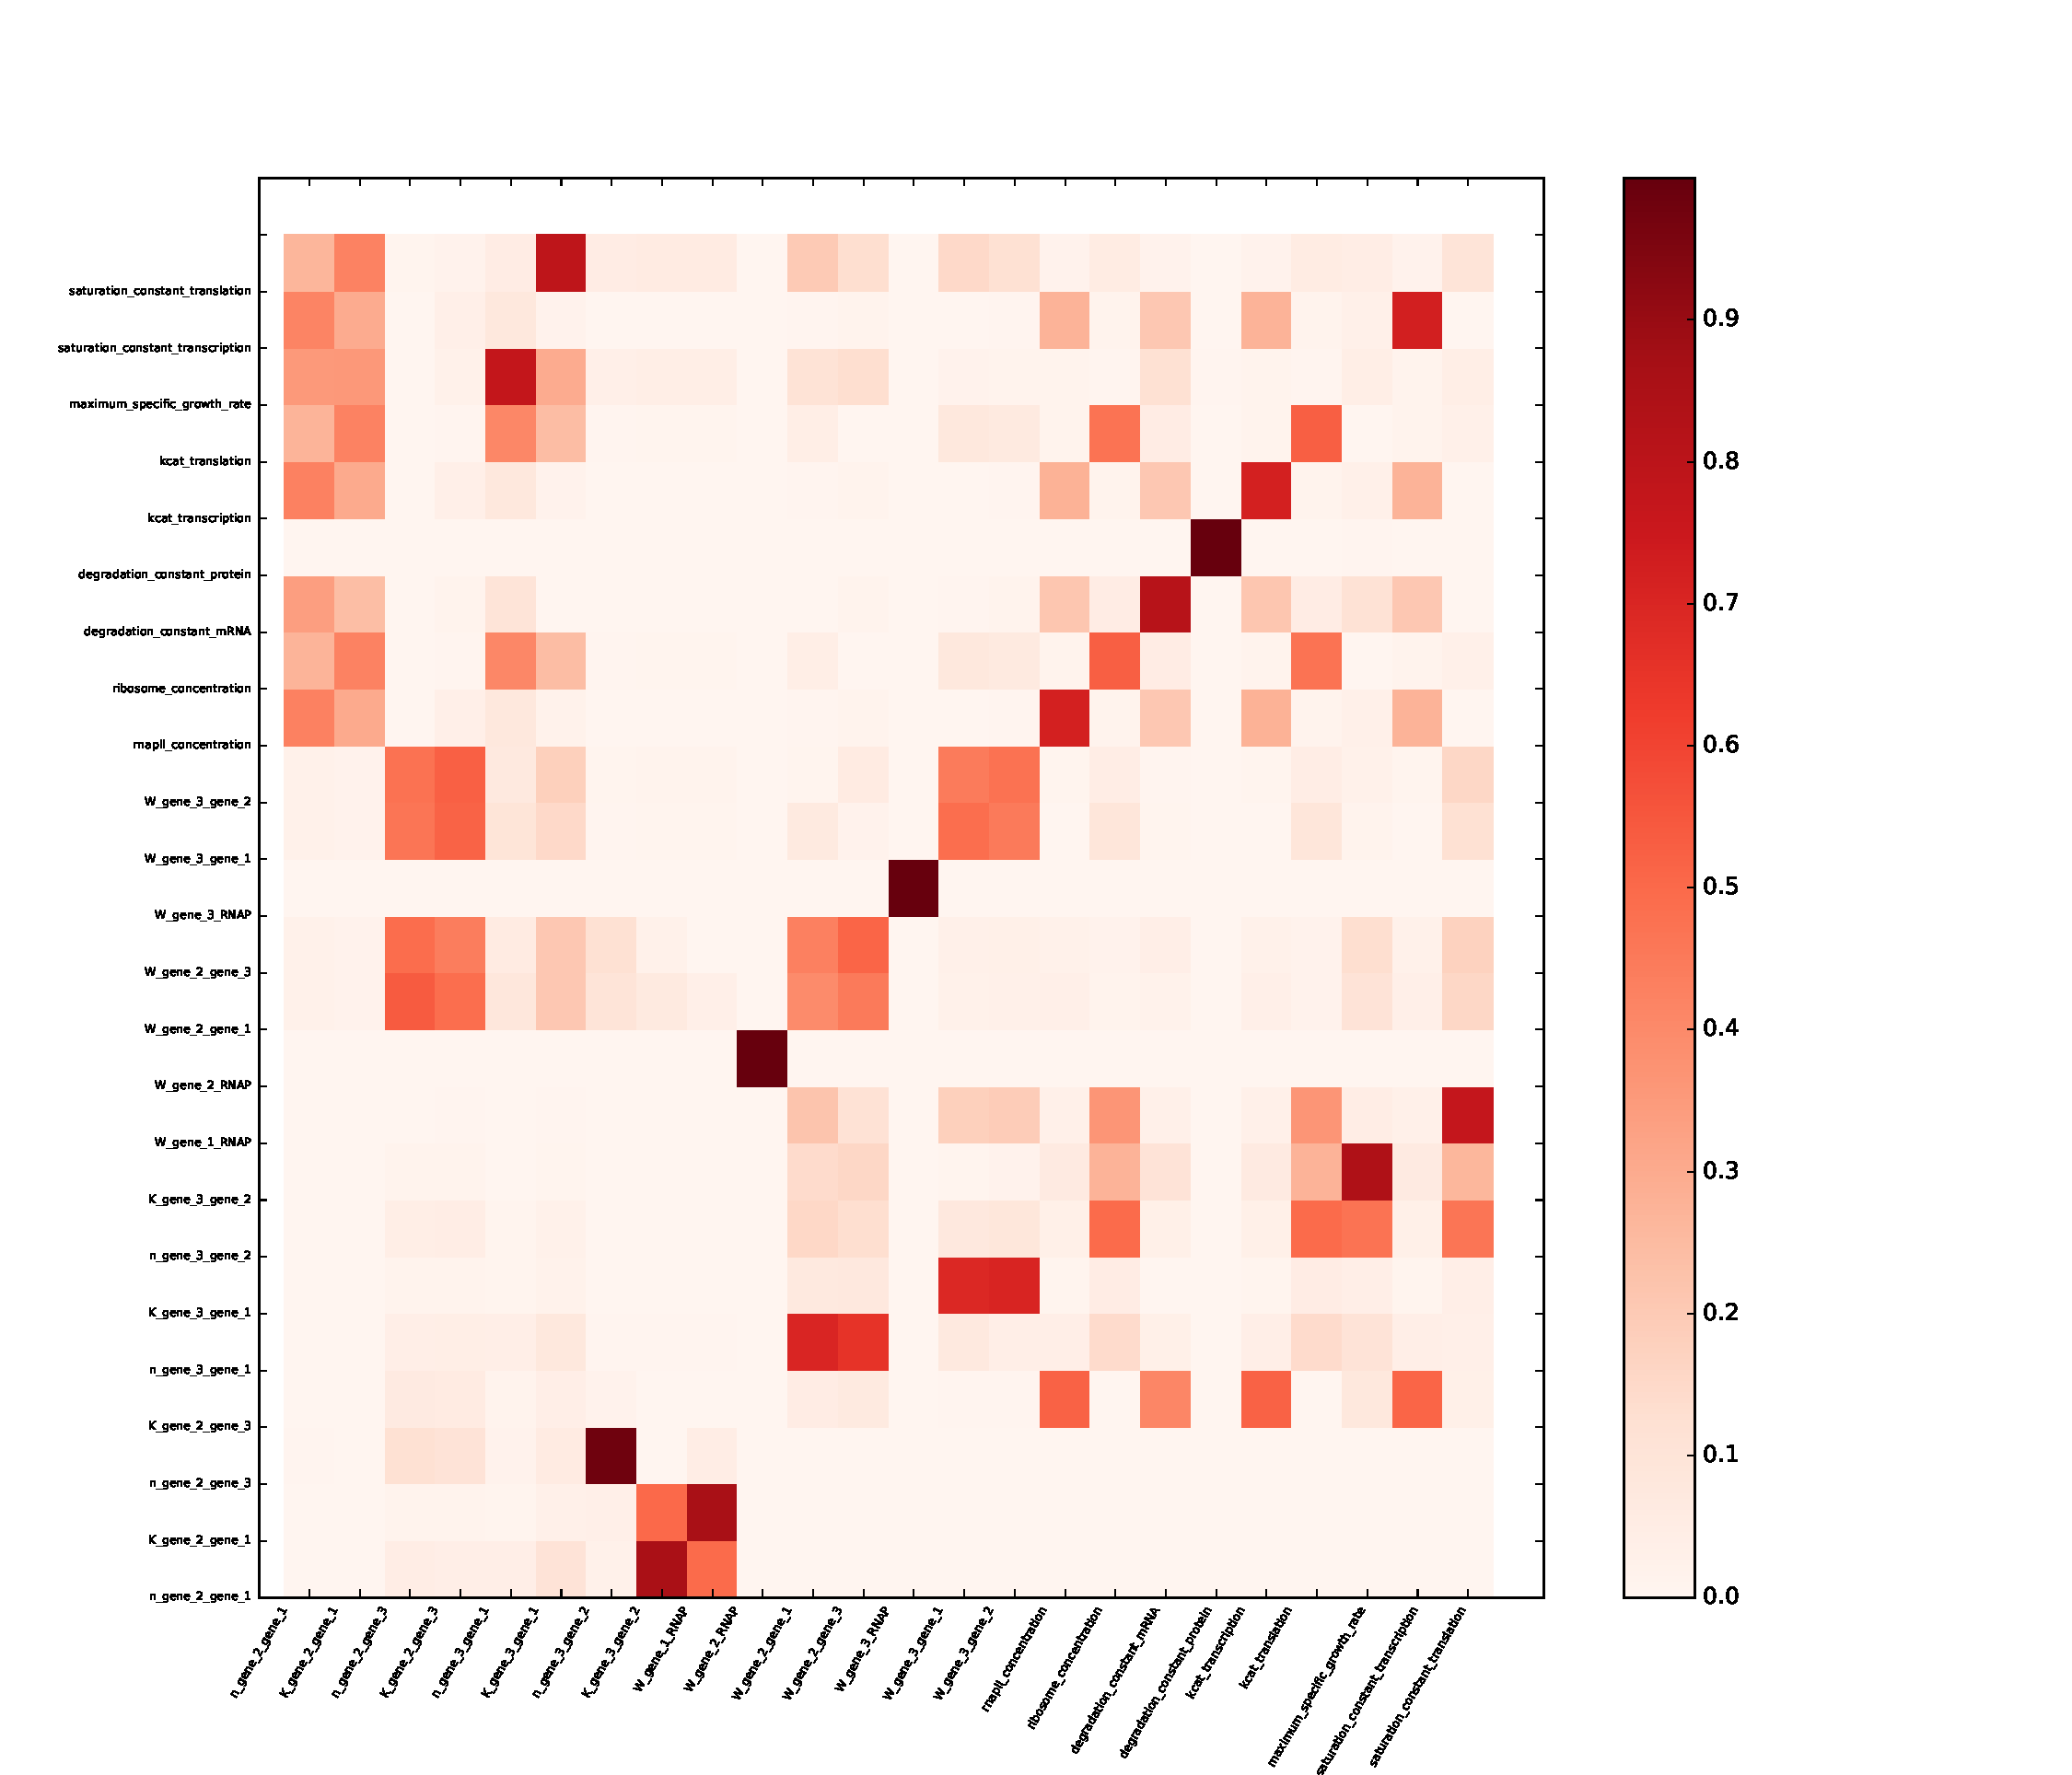
\includegraphics[width=12cm]{../ThreeGeneRachelV2/figures/ParameterInteractionsFrom10to70}
\caption{Heat map produced SVD of time averaged sensitivity of three gene network during induction showing parameter-parameter interactions}
\end{figure}
\end{document}